\definecolor{mygold}{RGB}{255,242,204}
\definecolor{myblue}{RGB}{219,238,243}

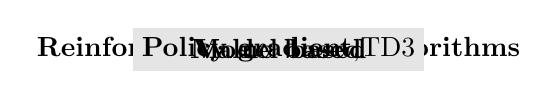
\begin{tikzpicture}[level distance=0.9in,sibling distance=.2in,scale=.65]
%\tikzset{edge from parent/.style= 
% {thick, draw,edge from parent fork right},every tree node/.style={draw,minimum width=1in,text width=1in, align=center},grow'=right}

\tikzset{edge from parent/.style= 
 {thick, draw, edge from parent fork down},
 every tree node/.style={draw,minimum width=1.5in,text width=1.2in,align=center,rounded corners=.2cm,,minimum height=0.4in},
 %gold subtree/.style = {fill={rgb:red,255;green,242;yellow,204}, draw, minimum width=1in, text width=1.2in, align=center, rounded corners=.2cm}
 %blue subtree/.style =  {fill={rgb:red,219;green,238;yellow,243}, draw, minimum width=1in, text width=1.2in, align=center, rounded corners=.2cm}
 grow'=down}

\Tree 
    [.\node[] {\textbf{Reinforcement learning \mbox{algorithms} }};
        [.\node[] {\textbf{Model free}};
            [.\node[fill=gray!20] {\textbf{Policy gradient}, \\ TD3}; ]
            [.\node[] {\textbf{Value based}}; ]
        ] 
        [.\node[] {\textbf{Model based}};]
    ]
\end{tikzpicture}